% !TEX root = ../main.tex
\vspace{-2mm}
\section{Inverse-distilled Diffusion Language Models}
\vspace{-2mm}
\label{sec:idlm}
  In this section, we present our core methodology for distilling a broad class of Diffusion Language Models into a few-step generator. Firstly, we provide the theoretical foundations supporting the extension of the Inverse Distillation framework to the discrete domain (\wasyparagraph\ref{sec:theoretical extension idlm}). We then address the practical challenges arising from the non-smooth nature of discrete spaces (\wasyparagraph\ref{sec:practical extension of idlm}). Lastly, we outline key implementation details (\wasyparagraph\ref{sec:technical aspects}).

\vspace{-2mm}
\subsection{Theoretical extension of Inverse Distillation}
\vspace{-1mm}
\label{sec:theoretical extension idlm}

\ecoparagraph{Unified notations.}
  SEDD~\eqref{eq:sedd loss}, MDLM~\eqref{eq:mdlm loss}, and Duo~\eqref{eq:duo loss} introduce different training objectives $\{\LC_{\text{SEDD}}, \LC_{\text{MDLM}}, \LC_{\text{Duo}}\}$ 
  and model parameterizations $\{\widehat{s}(x_t,t), \widehat{x}_0(x_t,t)\}$.
  To describe the distillation framework in a unified fashion, we use $\LC \in \{\LC_{\text{SEDD}}, \LC_{\text{MDLM}}, \LC_{\text{Duo}}\}$ to denote the diffusion training objective and introduce $\widehat{f}(x_t,t) \in \{\widehat{s}(x_t,t), \widehat{x}_0(x_t,t)\}$ as a parameterized function encompassing the relevant model parameterizations. Following the standard notation commonly adopted in diffusion distillation literature, we define the \textbf{teacher} model as:
  \begin{equation}
    f^* = \arg\min\nolimits_{\widehat{f}} \EE_{p^*(x_0)} \left[\LC(\widehat{f}, x_0)\right] \nonumber.
    \vspace{-1mm}
  \end{equation}

 \vspace{-0.2mm}
\ecoparagraph{Inverse distillation for DLMs.}
  To address the issue of slow inference, we extend the Inverse Distillation framework, originally developed for continuous diffusion models, to the domain of Diffusion Language Models.

  Specifically, we consider a \textbf{student} model defined by a generator ${G_{\theta}\colon \ZC \to \VC}$, parameterized by parameters $\theta$, which transforms latent variables from a latent space $\ZC$ to a discrete output space $\VC$. The latent space $\ZC$ is equipped with a tractable prior distribution $p_{\ZC}$, inducing a distribution $p_{\theta}$ over $\VC$ via the mapping $G_{\theta}$. Then, following the logic of the continuous case, we propose to consider the following objective for the discrete diffusion:
\vspace{-1mm}
  \begin{Box1}{IDLM loss}
    \vspace{-2pt}
    \begin{equation}
      \label{eq:inverse discrete diffusion distillation}
      \!\!\!\! \LC_{\text{IDLM}}(\theta) \vcentcolon= \mathop{\EE}_{p_{\theta}(x_0)} \! \Big[\LC(f^*, x_0)\Big]
      - \min_{\widehat{f}}\! \mathop{\EE}_{p_{\theta}(x_0)}\! \Big[\LC(\widehat{f}, x_0)\Big],\!
    \end{equation}
  \end{Box1}
  where the second term includes training of \textbf{fake} model using the same loss as the teacher model, but with data $p_{\theta}(x_0)$ produced by the generator $G_{\theta}$.

\ecoparagraph{Theoretical validity of the training objective.}
  However, simply formulating this objective in a manner analogous to the distillation loss used in continuous
  diffusion models does not guarantee the validity of its solutions. While the loss function admits a trivial minimizer
$\theta^*$ satisfying $p_{\theta^*} = p^*$, the absence of a uniqueness guarantee implies that the optimization procedure
may converge to suboptimal solutions. Consequently, it is essential to establish that the
\underline{minimizer recovers the true data distribution, i.e., ${p_{\theta^*} = p^*}$}. We present the following
theorem:

  \begin{theorem}[Unique solution]
%  \vspace{-1mm}
  \label{thm:unique solution} 
    For the SEDD~\eqref{eq:sedd loss}, MDLM~\eqref{eq:mdlm loss}, and Duo~\eqref{eq:duo loss} (in the limit as $\tau \to 0^{+}$) objectives the IDLM loss defined in equation~\eqref{eq:inverse discrete diffusion distillation} satisfies
    \begin{equation}
      \LC_{\text{IDLM}}(\theta) \geq \mathcal{D}_{\text{KL}}(p_{\theta} \parallel p^*)\geq 0 \nonumber
    \end{equation}
    and achieves its minimum (zero) if and only if the model distribution matches the target distribution
    \vspace{-2mm}
    \begin{equation}
      \LC_{\text{IDLM}}(\theta) = 0 \iff p_{\theta} = p^*. \nonumber
    \end{equation}
    \vspace{-2mm}
  \end{theorem}
  \vspace{-5mm}

  We give the proof in Appendix~\ref{app: proof of the theorem}.


  
  \begin{figure*}[ht!]
    \centering
    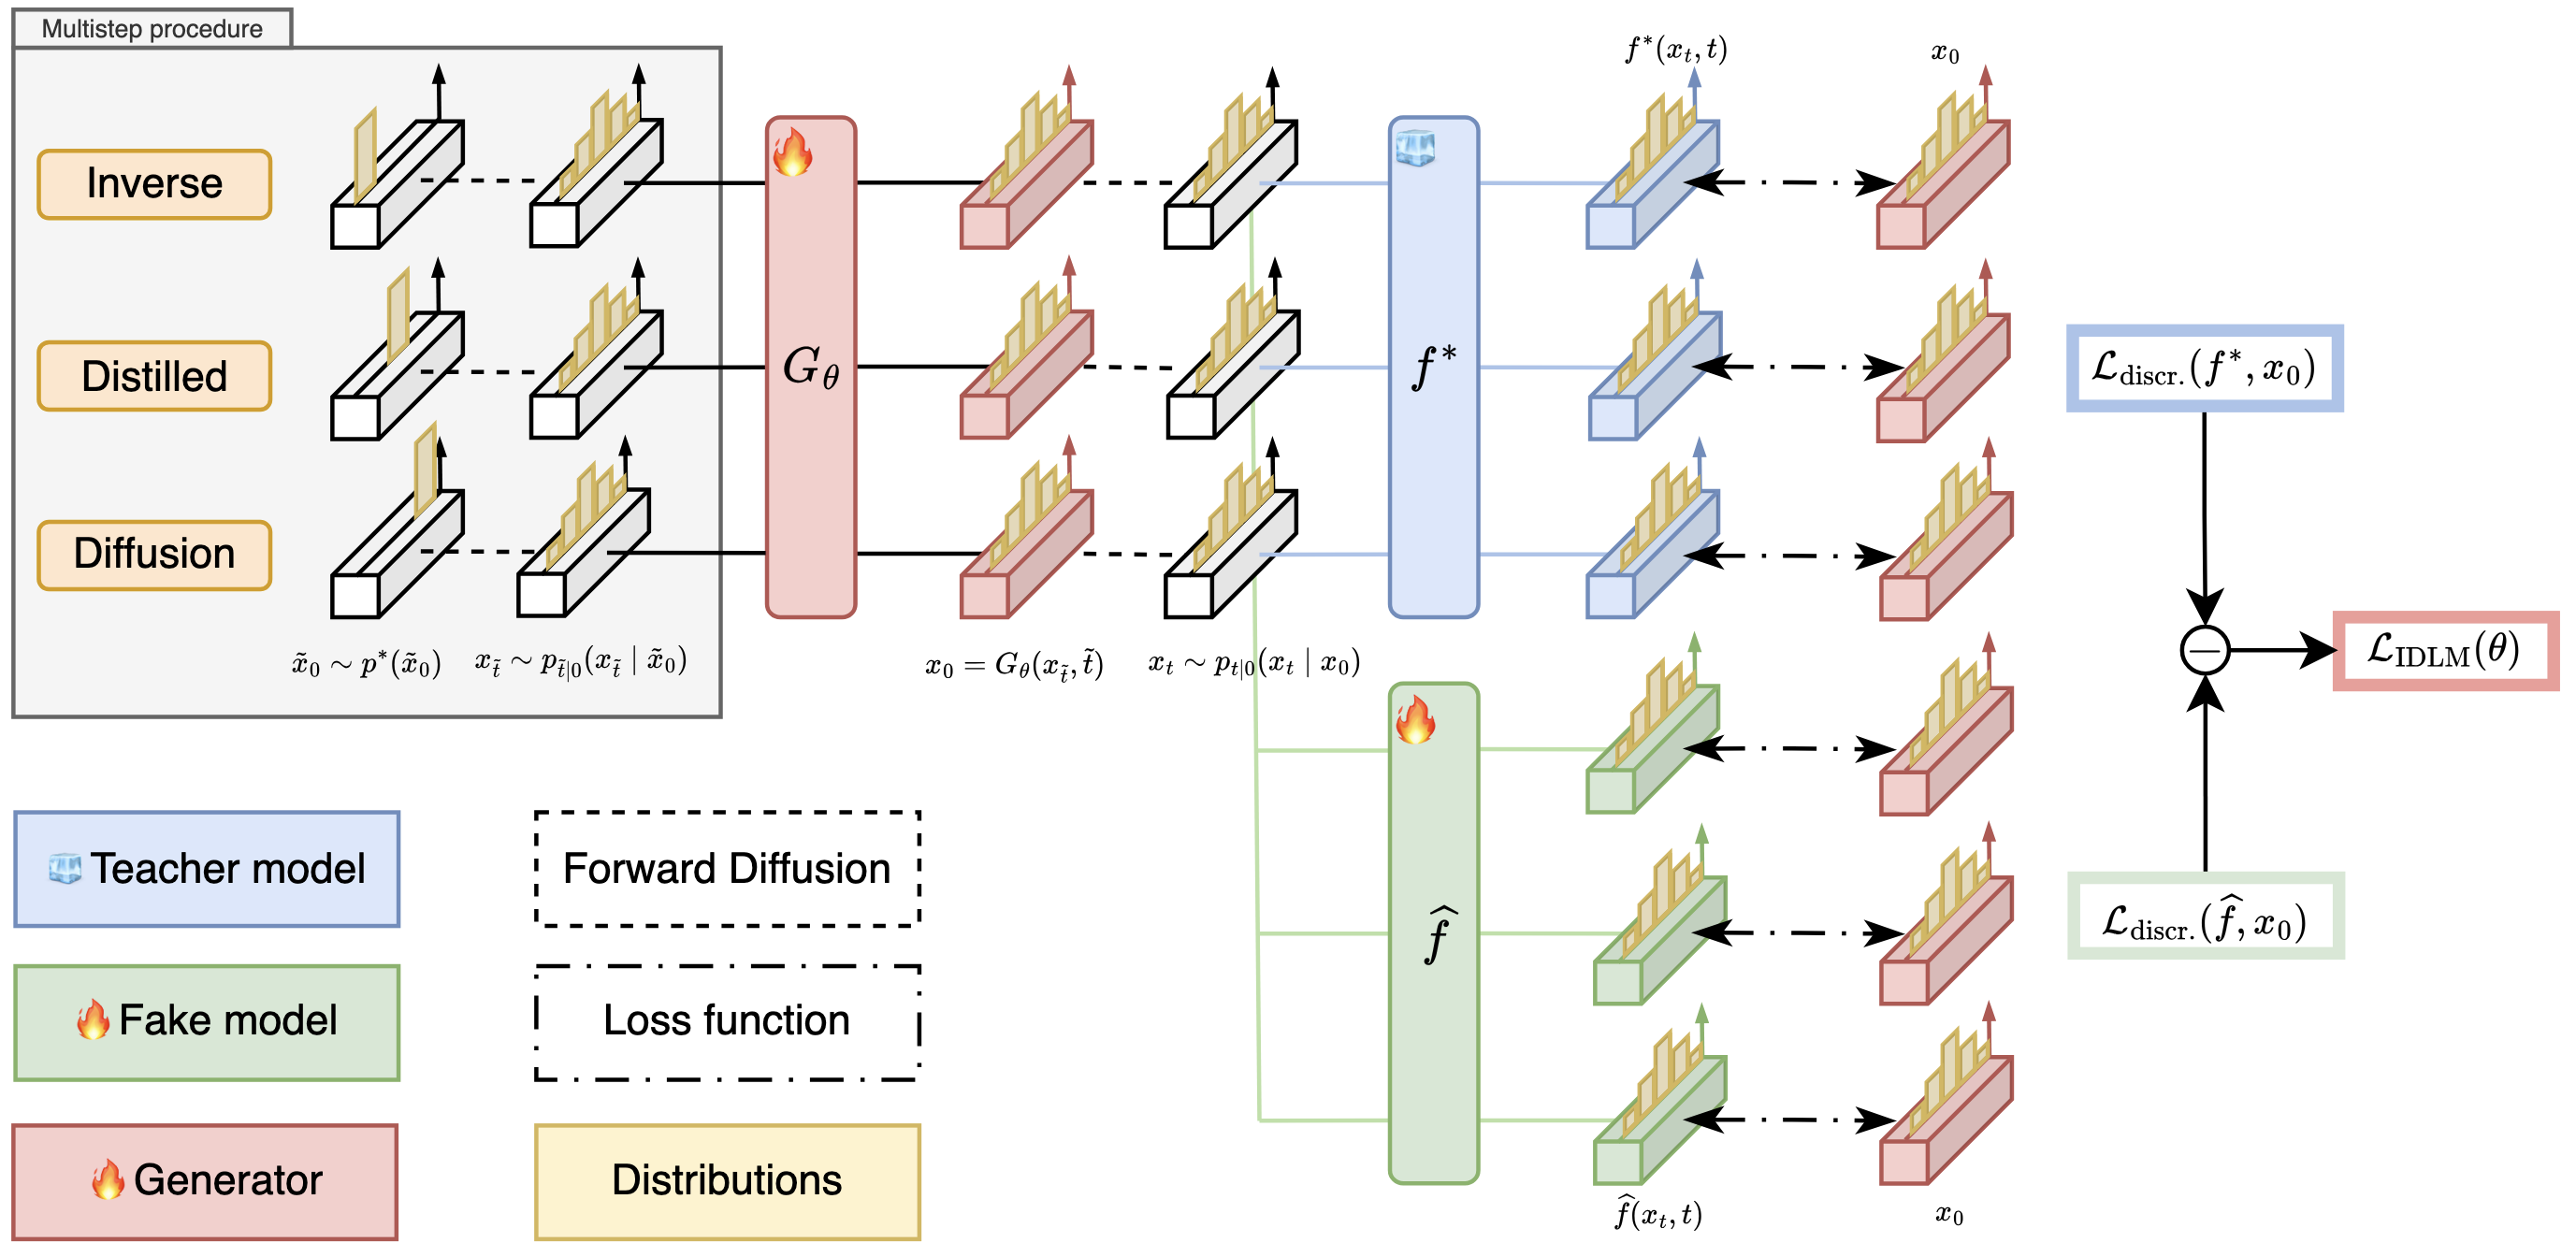
\includegraphics[width=0.82\linewidth]{ICLR2026_DeLTa/../images/method.png}
    \caption{\textbf{Overview of our Inverse-Distilled Diffusion Language Model (IDLM) framework.} The objective is to distill a pretrained Diffusion Language Model $f^*$, referred to as the \textbf{teacher}, into a few-step generator $G_{\theta}$, referred to as the \textbf{student}. To this end, we extend the concept of \emph{Inverse Distillation}, originally developed for continuous diffusion models, to the discrete domain. The training procedure involves a nested optimization scheme: an auxiliary diffusion model $\widehat{f}$ (the \textbf{fake} model), is optimized using the same training loss as the teacher, but with data generated by the student $G_{\theta}$. Subsequently, the generator is updated using the IDLM objective introduced in (\wasyparagraph\ref{sec:theoretical extension idlm}).}
%    \caption{\textbf{IDLM training.} Alternate between (i) fitting a fake model on student samples using the teacher loss and (ii) updating the generator to increase the teacher–fake loss gap on those samples.}
    \label{fig:method}
    \vspace{-4mm}
  \end{figure*}

% \label{sec:practical aspects}
%   While the theoretical foundations of the method have been established, a direct implementation of the IDLM loss for discrete diffusion models is not feasible in practice due to two primary challenges:
%   \begin{itemize}
%     \item The IDLM objective \eqref{eq:inverse discrete diffusion distillation} is not differentiable since it includes distribution $p_{\theta}$ parametrized by a discrete generator $G_{\theta}$. 
%     % gradients must pass through discrete sampling steps, $x_0 \sim p^{\theta}(x_0)$ and $x_t \sim p_{t \mid 0}(x_t \mid x_0)$.
%     \item Distilling teacher diffusion $f^*$ into a one-step generator $G_{\theta}$ for text generation, is practically challenging due to limited model capacity and the difficulty of learning a direct mapping from latent space to diverse, high-quality text.
%   \end{itemize}
%   %
%   To address these issues, we first propose a solution to the gradient estimation challenge in Section~\ref{sec:gradients}. Then, motivated by the second limitation, we extend the IDLM framework to support multi-step generation in Section~\ref{sec:multistep}. Finally, we summarize the method in Section~\ref{sec:algorithm}.

\vspace{-2mm}
\subsection{Practical extension of Inverse Distillation}
\label{sec:practical extension of idlm}
\vspace{-2mm}
Although we have theoretically established the validity of the proposed inverse distillation objective IDLM~\eqref{eq:inverse discrete diffusion distillation}, the discrete nature of the output space $\VC$ continues to pose significant practical challenges for the gradient-based optimization. 
In particular, the IDLM loss contains two primary bottlenecks. (i) First, the student generator ${G_{\theta} \colon \ZC \to \VC}$ produces outputs in the one-hot space $\VC$, which in practice necessitates the use of unstable techniques, such as the hard Gumbel-Softmax, thereby complicating gradient propagation. (ii) Second, samples $x_t \sim p_{t \mid 0}(x_t \mid x_0)$ depend on $x_0$, and thus implicitly on $\theta$. This introduces an additional challenge, as differentiating through the sampling operation $\sim$ is nontrivial in the discrete setting. Below we mitigate these challenges and develop a feasible training procedure.

\ecoparagraph{(i) Simplex relaxation.}
\label{sec:simplex relaxation}
To address the first challenge, we relax the output space of the student generator from the discrete set $\VC$ to the
probability simplex $\Delta$, and accordingly redefine the generator as $G_{\theta}\colon \ZC \to \Delta$.
This relaxation enables smooth gradient flow but introduces a nontrivial question regarding the computation of
the training objective, since the generator outputs no longer lie in the original discrete space. Specifically,
under this reparameterization, the $\LC_{\text{IDLM}}(\theta)$ objective becomes:
\begin{gather}
  \EE_{p_{\theta}(x_0)}\!\Bigl[\LC(f^*, x_0) - \min_{\widehat{f}}\LC(\widehat{f}, x_0)\Bigr]
  = \EE_{p_{\ZC}(z)}\!\Bigl[\LC(f^*, G_{\theta}(z)) - \min_{\widehat{f}}\LC(\widehat{f}, G_{\theta}(z))\Bigr],
  \nonumber
  \vspace{-2mm}
\end{gather}
where $z \sim p_{\ZC}(z)$ denotes a latent variable. Since $x_0$ appears only within the teacher loss $\LC$,
we must ensure that this loss remains computable when substituting discrete samples $x_0 \in \VC$ with relaxed
outputs $G_{\theta}(z) \in \Delta$. To this end, we note that all teacher losses under consideration
$\LC \in \{\LC_{\text{SEDD}}, \LC_{\text{MDLM}}, \LC_{\text{Duo}}\}$ incorporate $x_0$ in one of two
mathematically compatible forms: (i) through scalar products $\langle \cdot, x_0 \rangle$, or (ii) via the distribution
$p_{t|0}(\cdot \mid x_0)$, which can be expressed as a matrix-vector product:
\vspace{-1.5mm}
\begin{gather}
    p_{t \mid 0}(\cdot \mid x_0) = \exp\left(\bar{\sigma}_t Q\right)x_0.
    \nonumber
\end{gather}
%
Consequently, each of the considered teacher losses is mathematically well-defined not only for one-hot vectors
from $\VC$ but also for any input from the probability simplex $\Delta$. This reparameterization enables end-to-end
training of the generator using standard differentiable operations, such as the $\softmax$ function, by avoiding
the need for unstable discrete relaxation like the Gumbel--Softmax.


\textbf{Case of Duo.} The training objective in the Duo setting is given in equation~\eqref{eq:duo loss} as
\begin{gather}
  \textstyle \LC_{\text{Duo}}(\widehat{x}_0, x_0)\vcentcolon=
  \int_0^1 \EE_{\tilde{p}_{t\mid 0}(w_t\mid x_0)} \left[g(x_t(w_t),x_0, \widehat{x}_0(x_t^{\tau}(w_t), t))\right]dt. \nonumber
\end{gather}
Here we can apply the standard reparameterization trick for Gaussians by expressing the latent variable $w_t$ as
%\vspace{-1mm}
%\begin{gather}
$
  \textstyle w_t(x_0, \epsilon) = \tilde{\alpha}_t x_0 + \sqrt{1 - \tilde{\alpha}_t^2} \, \epsilon,
  $
%\end{gather}
where $\epsilon \sim \NC(0, I)$ is sampled independently of $x_0$. Substituting this into the objective yields
\begin{gather}
  \textstyle \LC_{\text{Duo}}(\widehat{x}_0, x_0)\vcentcolon=
  \int_0^1 \EE_{\epsilon \sim \NC(0, I)} \, \left[g(x_t(w_t),x_0, \widehat{x}_0(x_t^{\tau}(w_t), t))\right] \, dt,
\end{gather}
which eliminates the need to differentiate through the sampling operation itself, as the randomness is now isolated in $\epsilon$, which is independent of $x_0$. This reparameterization thus enables gradient-based optimization of the Duo objective.


\textbf{Case of MDLM (SEDD absorbing).} In the case of MDLM, the forward transition distribution $p(x_t \mid x_0)$ does not admit a standard reparameterization. However, we can leverage the \textsc{subs} parameterization of the MDLM model introduced in~\citep[see Section 3.2.3]{sahoo2024simple}. Specifically, for unmasked tokens (i.e., $x_t \neq m$), the following properties hold: (a) the optimal denoiser satisfies $\widehat{x}_0(x_t, t) = x_t$, and (b) $x_t = x_0$, since the forward process either preserves the token or replaces it with a fixed mask token $m$. As a result, in this case, $\widehat{x}_0(x_t, t) = x_t = x_0$, and the loss becomes $\LC_{\text{MDLM}}(x_0, x_0) = 0.$
Thus, all nonzero contributions to the loss arise from instances where $x_t = m$. In this case, $x_t$ is independent of $x_0$, as the mask token is fixed and does not result from a stochastic transformation conditioned on $x_0$. Consequently, there is no need to backpropagate through the sampling of $p_{t \mid 0}(x_t \mid x_0)$. This allows us to rewrite the loss as:
\begin{gather}
  \textstyle \int_0^1 \, \EE_{p_{t \mid 0}(x_t \mid \text{sg}(G_{\theta}(z)))} \left[
  \lambda_t \, \langle \log \widehat{x}_0(x_t, t), G_{\theta}(z) \rangle
  \right] dt,
  \nonumber
\end{gather}
where $\text{sg}(\cdot)$ denotes the stop-gradient operator. This formulation enables efficient training without requiring differentiable sampling from the discrete forward process.


\vspace{-1mm}
\subsection{Technical Aspects}
\label{sec:technical aspects}
\vspace{-1mm}
\ecoparagraph{Models initialization.}
    Following prior distillation approaches that employ an auxiliary fake model during training~\citep{yin2024one, yin2024improved, zhou2024score, zhou2024adversarial, gushchin2025inverse, kornilov2025universal}, we initialize both the fake diffusion model and the student generator using the parameters of the pretrained teacher diffusion model.

\ecoparagraph{Multistep distillation.}
    We distill a \(K\)-step student that conditions on \((x_t,t)\) and initialize it from the teacher for stability. Full parameterization and training details are in Appendix~\ref{app:method_details}.

%We observe that distilling a single-step generator for text generation remains practically challenging. This observation motivates us to follow prior works~\citep{yin2024one, yin2024improved, gushchin2025inverse} and extend the IDLM framework to support multistep generation. To enable few-step inference, and given that the student generator is initialized from the pretrained teacher model, we adopt the same latent space $\ZC$ as for the teacher. Therefore, the generator is parameterized as $G_{\theta} \colon \VC \times [0, 1] \to \Delta$ in the SEDD and MDLM settings, and as $G_{\theta} \colon \Delta \times [0, 1] \to \Delta$ in the Duo setting. To avoid notational ambiguity, we denote samples from the target data distribution as $\tilde{x}_0 \sim p^*(\tilde{x}_0)$. Under this parameterization, the generator receives as input either: (i) samples $x_{\tilde{t}} \sim p_{\tilde{t} \mid 0}(x_{\tilde{t}} \mid \tilde{x}_0)$ in the SEDD and MDLM settings, or (ii) soft embeddings $x_{\tilde{t}}^{\tau}(w_{\tilde{t}}(\tilde{x}_0, \epsilon))$ in the Duo setting, where $\epsilon \sim \mathcal{N}(0, I)$ and $\tilde{x}_0 \sim p^*(\tilde{x}_0)$ is drawn from the data distribution.
%    This design enables the generator to leverage supervision from ground-truth data samples, which can lead to improved generation quality. As a result, the generator is capable of performing multistep inference in the same manner as the teacher model, by numerically integrating the reverse-time dynamics~\eqref{eq:backward diffusion}.


\ecoparagraph{Training of fake model.}
    The proposed IDLM loss function involves an inner optimization with respect to the fake model.
    To approximate this nested optimization in practice, we adopt an alternating training scheme,
%    following prior works~\citep{yin2024one, yin2024improved, zhou2024score, zhou2024adversarial, gushchin2025inverse, kornilov2025universal}.
    following prior works~\citep{yin2024one, yin2024improved, gushchin2025inverse, kornilov2025universal}.
Specifically, training proceeds by alternating between 2 optimization steps.

    (i) \underline{Updating the fake model} $\widehat{f}$ while keeping the student generator $G_{\theta}$ fixed. In this step, the fake model is optimized using the teacher loss $\LC$ evaluated on samples generated by the student. Taking into account the multistep training procedure, for a fixed sample $x_{\tilde{t}} \sim p_{\tilde{t} \mid 0}(x_{\tilde{t}} \mid \tilde{x}_0)$ with $\tilde{x}_0 \sim p^*(\tilde{x}_0)$, the resulting optimization objective for updating the fake model is given by:
    \vspace{-1mm}
    \begin{gather}
    \label{eq:update fake in practice}
      \text{\textit{Update:} } \widehat{f} \text{;} \quad \text{\textit{Fix:} } \theta  \\
      \LC_{\widehat{f}} = \! \LC(\widehat{f}, G_{\theta}(x_{\tilde{t}}, \tilde{t})). \nonumber
    \vspace{-1mm}
    \end{gather}
    (ii) \underline{Updating the student generator} $G_{\theta}$ while keeping the fake model $\widehat{f}$ fixed. Considering the multistep training procedure, for a fixed sample $x_{\tilde{t}} \sim p_{\tilde{t} \mid 0}(x_{\tilde{t}} \mid \tilde{x}_0)$ with $\tilde{x}_0 \sim p^*(\tilde{x}_0)$, the IDLM loss~\eqref{eq:inverse discrete diffusion distillation} can be instantiated as:
    \vspace{-2mm}
    \begin{gather}
        \label{eq:update generator in practice}
        \text{\textit{Update:} } \theta \text{;} \quad \text{\textit{Fix:} } \widehat{f} \\
        \LC_{\text{IDLM}}(\theta) \!=\! \LC(f^*, G_{\theta}(x_{\tilde{t}}, \tilde{t}))-
      \! \LC(\widehat{f}, G_{\theta}(x_{\tilde{t}}, \tilde{t})). \nonumber
    \end{gather}
    %\vspace{-1mm}
    
\vspace{-3mm}
\ecoparagraph{Algorithm.}
  In summary, Algorithm~\ref{alg:idlm} outlines the proposed procedure for distilling a pretrained DLM into a few-step generator using the IDLM objective. A visual illustration of the method is provided in Figure~\ref{fig:method}.
